\documentclass{standalone}
\usepackage{tikz}
\usetikzlibrary{positioning,shapes}
\begin{document}
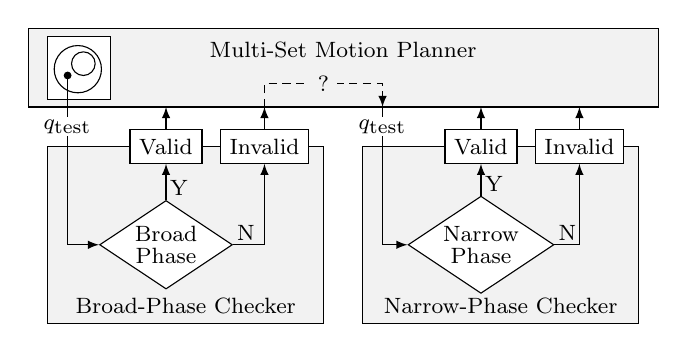
\begin{tikzpicture}

\tikzstyle{every node}=[font=\footnotesize]
\tikzset{>=latex} % arrow heads

\node[draw,rectangle,fill=black!5,
  inner sep=0,minimum width=8cm,minimum height=1.0cm]
  (boxmp) at (4,-0.5) {};
\node[above = -0.5cm of boxmp] {Multi-Set Motion Planner};

% c-space depiction
\node[draw,fill=white,rectangle,
   minimum width=0.8cm,minimum height=0.8cm] at (0.65,-0.5) {};
\draw (0.63,-0.52) circle [radius=0.3cm];
\draw (0.70,-0.45) circle [radius=0.15cm];
\node[circle,fill=black,inner sep=1.0] at (0.5,-0.6) {};

\node[draw,rectangle,fill=black!5,
  minimum width=3.5cm,minimum height=2.25cm]
  (boxcc) at (2,-2.625) {};
\node[below = -0.45cm of boxcc] {Broad-Phase Checker};

\node[draw,rectangle,fill=black!5,
  minimum width=3.5cm,minimum height=2.25cm]
  (boxcc) at (6,-2.625) {};
\node[below = -0.45cm of boxcc] {Narrow-Phase Checker};

\node[draw,fill=white,diamond,aspect=1.5,align=center,
  inner sep=1]
  (bp) at (1.75,-2.75) {Broad\\[-0.05cm]Phase};

\node[draw,fill=white,diamond,aspect=1.5,align=center,
  inner sep=1]
  (np) at (5.75,-2.75) {Narrow\\[-0.05cm]Phase};

\node[draw,fill=white,rectangle] (bv) at (1.75,-1.5) {Valid};
\node[draw,fill=white,rectangle] (bi) at (3.0,-1.5) {Invalid};

\node[draw,fill=white,rectangle] (nv) at (5.75,-1.5) {Valid};
\node[draw,fill=white,rectangle] (ni) at (7.0,-1.5) {Invalid};

\draw[->] (0.5,-0.6) -- (0.5,-2.75) -- (bp.west);
\draw[->] (bp.north) -- (bv.south);
\draw[->] (bv.north) -- (1.75,-1.0);
\draw[->] (bp.east) -- (3.0,-2.75) -- (bi.south);
\draw[->] (bi.north) -- (3.0,-1.0);

\draw[densely dashed] (3.0,-1.0) -- (3.0,-0.7) -- (3.6,-0.7);
\draw[->,densely dashed] (3.9,-0.7) -- (4.5,-0.7) -- (4.5,-1.0);

\draw[->] (4.5,-1.0) -- (4.5,-2.75) -- (np.west);
\draw[->] (np.north) -- (nv.south);
\draw[->] (nv.north) -- (5.75,-1.0);
\draw[->] (np.east) -- (7.0,-2.75) -- (ni.south);
\draw[->] (ni.north) -- (7.0,-1.0);

\node[rectangle,fill=black!5,inner sep=3] at (3.75,-0.7) {?};

\node[rectangle,fill=white,inner sep=1] at (0.5,-1.25)
  {$q_{\mbox{\scriptsize test}}$};
\node[rectangle,fill=white,inner sep=1] at (4.5,-1.25)
  {$q_{\mbox{\scriptsize test}}$};

\node[above right = -0.1cm of bp.north] {Y};
\node[above right = -0.1cm of bp.east] {N};
\node[above right = -0.1cm of np.north] {Y};
\node[above right = -0.1cm of np.east] {N};

%\draw[step=1,black!10,very thin] (0,-4) grid (8,0);

\end{tikzpicture}%
\end{document}
